%iffalse
\let\negmedspace\undefined
\let\negthickspace\undefined
\documentclass[journal,12pt,onecolumn]{IEEEtran}
\usepackage{cite}
\usepackage{amsmath,amssymb,amsfonts,amsthm}
\usepackage{algorithmic}
\usepackage{graphicx}
\usepackage{textcomp}
\usepackage{xcolor}
\usepackage{txfonts}
\usepackage{listings}
\usepackage{enumitem}
\usepackage{mathtools}
\usepackage{gensymb}
\usepackage{comment}
\usepackage[breaklinks=true]{hyperref}
\usepackage{tkz-euclide} 
\usepackage{listings}
\usepackage{gvv}                                        
%\def\inputGnumericTable{}                                 
\usepackage[latin1]{inputenc}                                
\usepackage{color}                                            
\usepackage{array}                                            
\usepackage{longtable}                                       
\usepackage{calc}                                             
\usepackage{multirow}                                         
\usepackage{hhline}                                           
\usepackage{ifthen}                                           
\usepackage{lscape}
\usepackage{tabularx}
\usepackage{array}
\usepackage{float}
\usepackage{multicol}
\usepackage{subcaption}

\newtheorem{theorem}{Theorem}[section]
\newtheorem{problem}{Problem}
\newtheorem{proposition}{Proposition}[section]
\newtheorem{lemma}{Lemma}[section]
\newtheorem{corollary}[theorem]{Corollary}
\newtheorem{example}{Example}[section]
\newtheorem{definition}[problem]{Definition}
\newcommand{\BEQA}{\begin{eqnarray}}
\newcommand{\EEQA}{\end{eqnarray}}
\newcommand{\define}{\stackrel{\triangle}{=}}
\theoremstyle{remark}
\newtheorem{rem}{Remark}


% Marks the beginning of the document
\begin{document}
\bibliographystyle{IEEEtran}
\vspace{3cm}

\title{NCERT-9.5.2}
\author{S. Sai Akshita - EE24BTECH11054}
\newpage
\maketitle
\bigskip

\renewcommand{\thefigure}{\theenumi}
\renewcommand{\thetable}{\theenumi}
\textbf{Question:}
Find the general solution of the Differential Equation
\begin{align}
\frac{dy}{dx} + 3y = e^{-2x} \label{eq:1}
\end{align}
\textbf{Obtaining Solution using Integrating Factor:}
The given Differential Equation is a first-order linear equation of the form:
\begin{align}
\frac{dy}{dx} + p\brak{x}\times y = q\brak{x}
\end{align}
The Integrating Factor for such equations is given by:
\begin{align}
\text{IF} = e^{\int p\brak{x}dx}
\end{align}
For this question, it is:
\begin{align}
\text{IF} = e^{\int 3dx} = e^{3x}
\end{align}
Multiplying the entire equation \eqref{eq:1} by the Integrating Factor , we get:
\begin{align}
\frac{dy}{dx} e^{3x} + 3y e^{3x} &= e^{3x} e^{-2x} \\
\frac{d}{dx}\brak{ye^{3x}} &= e^{x}
\end{align}
Integrating both sides:
\begin{align}
\int \frac{d}{dx}\brak{ye^{3x}} dx &= \int e^{x} dx \\
ye^{3x} &= e^{x} + C
\end{align}
Dividing through by :
\begin{align}
y &= e^{-2x} + Ce^{-3x} \label{eq:2}
\end{align}
Thus, \eqref{eq:2} is the general solution of the given Differential Equation.\\
Assume $c=1$. The solution becomes:
\begin{align}
y = e^{-2x} + e^{-3x} \label{eq:3}
\end{align}
From here, initial conditions=$\brak{x_0,y_0}=\brak{0,2}$\\
\textbf{Obtaining solution by Laplace Transform:}\\
The fundamental formula for Laplace Transform is:\\
\begin{align}
    \mathcal{L}\brak{f\brak{t}} = F\brak{s} = \int_{0}^{\infty} e^{-st} f\brak{t}  dt
\end{align}
Taking the Laplace transform on both sides of \ref{eq:1}
\begin{align}
    \mathcal{L}\brak{\frac{dy}{dx}} + 3\mathcal{L}\brak{y} = \mathcal{L}\brak{e^{-2x}}
\end{align}
Using the Laplace transform properties:
\begin{align}
    \mathcal{L}\brak{\frac{dy}{dx}} = sY\brak{s} - y\brak{0}, \quad \mathcal{L}\brak{y} = Y\brak{s}, \quad \mathcal{L}\brak{e^{-2x}} = \frac{1}{s + 2}.
\end{align}
Substituting these into the equation:
\begin{align}
sY\brak{s} - 2 + 3Y\brak{s} = \frac{1}{s + 2}.
\end{align}
After simplification,
\begin{align}
    Y\brak{s} = \frac{1}{\brak{s + 3}\brak{s + 2}} + \frac{2}{s + 3}.
\end{align}
Applying partial fractions to the first term of above equation,
\begin{align}
\frac{1}{\brak{s + 3}\brak{s + 2}} &= \frac{A}{s + 3} + \frac{B}{s + 2}.\\
1 &= A\brak{s + 2} + B\brak{s + 3}.\\
1 &= A\brak{s} + 2A + B\brak{s} + 3B.\\
1 &= \brak{A + B}s + \brak{2A + 3B}.
\end{align}
By comparing the coefficients, we get
\begin{align}
A + B &= 0 \\
2A + 3B &= 1
\end{align}
Solving this system of equations:
\begin{align}
B &= -A, \\
2A + 3\brak{-A} &= 1 \\ 
B = -A &= 1.
\end{align}
Thus:
\begin{align}
\frac{1}{\brak{s + 3}\brak{s + 2}} = \frac{-1}{s + 3} + \frac{1}{s + 2}.
\end{align}
Substitute back into $ Y\brak{s} $:
\begin{align}
    Y\brak{s} &= \frac{-1}{s + 3} + \frac{1}{s + 2} + \frac{2}{s + 3}\\
    Y\brak{s} &= \frac{1}{s + 3} + \frac{1}{s + 2}.
\end{align}
\textbf{Finding the Region of Convergence (ROC):}\\
Each term in $Y\brak{s}$ contributes a pole:
The term $\frac{1}{s+3}$ has a pole at $s = -3$, and the term $\frac{1}{s+2}$ has a pole at $s = -2$.Thus, the poles of $Y\brak{s}$ are located at $s = -3$ and $s = -2$.\\\\
The ROC of a Laplace transform depends on whether the signal is:
\begin{enumerate}
    \item \textbf{Right-sided (causal):} The ROC is to the right of the rightmost pole, i.e., $ \text{Re}(s) > -2 .$
    \item \textbf{Left-sided (anti-causal):} The ROC is to the left of the leftmost pole, i.e., $ \text{Re}(s) < -3 .$
    \item \textbf{Two-sided:} The ROC lies between the poles, i.e., $-3 < \text{Re}(s) < -2 .$
\end{enumerate}
To determine the exact ROC, additional information about the time-domain behavior of the signal is needed:
\begin{enumerate}
    \item For a \textbf{causal signal}, the ROC is:
    $ \text{Re}(s) > -2. $
    \item For an \textbf{anti-causal signal}, the ROC is:
    $\text{Re}(s) < -3. $
    \item For a \textbf{two-sided signal}, the ROC is:
    $ -3 < \text{Re}(s) < -2. $
\end{enumerate}
The ROC depends on the nature of the signal (causal, anti-causal, or two-sided).\\
In causal systems, The function $y\brak{x}$ depends only on present and past values $\brak{x\geq0}$.
\\\\Using the inverse Laplace transform:
\begin{align}
    \mathcal{L}^{-1}\brak{\frac{1}{s + a}} = e^{-ax}.
\end{align}
Substituting in the above equation  :
\begin{align}
y\brak{x} &= \mathcal{L}^{-1}\brak{\frac{1}{s + 3}} + \mathcal{L}^{-1}\brak{\frac{1}{s + 2}}\\
y\brak{x} &= e^{-3x} + e^{-2x}
\end{align}
The Laplace Transform converts linear differential equations with constant coefficients into simpler algebraic equations in the Laplace domain.This simplification makes complex systems easier to analyze and solve.\\
\textbf{Plotting the Curve:}
To trace the curve, we calculate the slope of the tangent, at a point  on the curve. From \eqref{eq:1}, the slope is given by:
\begin{align}
\frac{dy}{dx} = e^{-2x} - 3y
\end{align}
Using this slope, we calculate successive points along the curve using a small step size :
\begin{align}
x_1 &= x_0 + h, \\
y_1 &= y_0 + h \frac{dy}{dx}\bigg|_{\brak{x_0, y_0}}
\end{align}
Similarly, for subsequent points:
\begin{align}
x_2 &= x_1 + h, \\
y_2 &= y_1 + h \frac{dy}{dx}\bigg|_{\brak{x_1, y_1}}
\end{align}
For generating $\brak{n+1}^{th}$ point, 
\begin{align}
    x_{n+1}&=x_n + h\\
    y_{n+1}&=y_n + h\times\brak{e^{-2x_n} - 3y_n} \\
    y_{n+1}&=y_{n}\brak{1-3h}+he^{-2x_{n}}
\end{align}
Repeating this process for a large number of points, we can trace the curve that represents one of the solutions of the Differential Equation.
To generate the plot, start from an initial point  satisfying \eqref{eq:3}, choose a small value of $h$, and calculate successive points,using the equations mentioned above.

\begin{figure}[h]
    \centering
    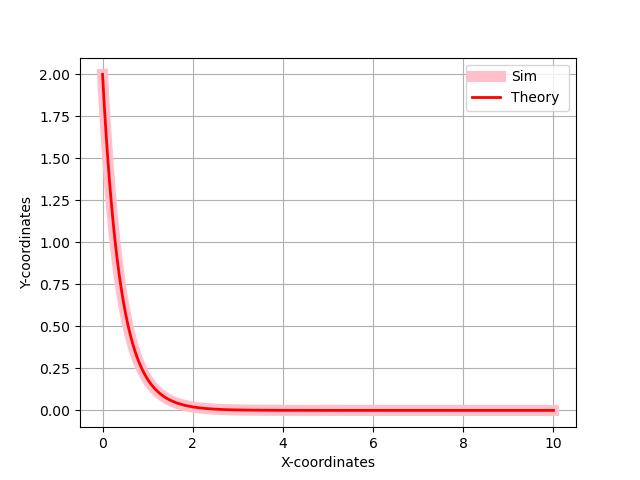
\includegraphics[width=\columnwidth]{Graph.jpeg}
    \label{fig:example}
\end{figure}



   
\end{document}
